\section{Parallel Machine Models} \label{sec:6}

\subsection{Makespan without Constraints} \label{subsec:6.1}
The makespan is not a very interesting objective for a single machine. 
However, for parallel machine models, minimizing the makespan has the effect 
of balancing the load over the various machines, which is an important 
objective in practice. Recall that we denote this by $(P_m~\|~C_{\max})$.

One can see that $(P_2~\|~C_{\max})$ is $\NP$-hard via a reduction from 
\textsc{Partition}. Indeed, consider an instance of \textsc{Partition}, 
where we are given $a_1, \dots, a_t \in \Z^+$ and want to find a subset 
$S \subseteq \{1, \dots, t\}$ such that 
\[ \sum_{j\in S} a_j = \frac12 \sum_{j=1}^t a_j = b. \] 
Let $n = t$ be the number of jobs each with processing time $p_j = a_j$. Then 
it is easy to check that there is a schedule with optimal value at most 
$\frac12 \sum_{j=1}^n p_j$ if and only if there is a solution to the 
\textsc{Partition} instance. 

Over the years, there have been many heuristics developed for 
$(P_m~\|~C_{\max})$. We focus on one such heuristic, and present it by 
discussing some history on how this algorithm was developed. First, we 
take a look at the list scheduling rule, which runs in $O(n\log m)$ time 
using a priority queue for the loads. 

\begin{algo}[List Scheduling]{algo:6.1}
    Given $n$ jobs in some arbitrary order, assign job $j$ to machine $i$ 
    whose load is smallest so far for each $j \in [n]$. 
\end{algo}

There are two obvious lower bounds on OPT, namely 
\begin{enumerate}[(1)]
    \item $\text{OPT} \geq \max_{j\in[n]} p_j$ since the jobs are not preemptive, and 
    \item $\text{OPT} \geq \frac1m \sum_{j=1}^n p_j$ because at least one machine must 
    have load which is at least the average. 
\end{enumerate}
We shall denote the load of a machine $i$ by $L(i) = p(S(i)) = 
\sum_{j\in S(i)} p_j$, where $S(i)$ is the set of jobs assigned to machine $i$.

\begin{theo}{theo:6.2}
    Algorithm~\ref{algo:6.1} is a $2$-approximation for $(P_m~\|~C_{\max})$. 
\end{theo}
\begin{pf}
    Let $i$ denote the machine which the highest load determining the objective 
    value. Let $j$ be the last job scheduled on machine $i$. When job $j$ was 
    assigned to machine $i$, it had the smallest load. Its load before the 
    assignment was $L(i) - p_j$, and thus $L(i) - p_j \leq L(k)$ for all 
    $1 \leq k \leq m$. Summing up this inequality over all $k$ and 
    dividing by $m$, we obtain 
    \[ L(i) - p_j \leq \frac1m \sum_{k=1}^m L(k) = \frac1m \sum_{j=1}^n p_j 
    \leq \text{OPT}. \] 
    We deduce that $L(i) = (L(i) - p_j) + p_j \leq 2 \cdot \text{OPT}$. 
\end{pf}

Is this analysis tight? That is, are there any examples where the factor 
is as bad as $2$? The answer is essentially yes. Suppose there are $m$ machines.
Take $m(m-1)$ jobs each with processing time $1$, and let the last job 
in the order have processing time $m$. Then the list scheduling algorithm 
will try to balance the $m(m-1)$ jobs among the $m$ machines first. Then 
we are forced to run the last job with processing time $m$ last on one 
of the machines, and that machine has load $2m - 1$. An optimal schedule 
instead places the job with processing time $m$ on its own machine, 
and balances the load of the $m(m-1)$ jobs between the remaining $m-1$ 
machines. This gives a makespan of $m$ instead. 

It can be shown that Algorithm~\ref{algo:6.1} is in fact a 
$(2 - \frac1m)$-approximation, and the above example shows that this is 
exactly a tight bound. 

We now consider the {\bf Longest Processing Time first (LPT)} rule.

\begin{algo}[LPT]{algo:6.3}
    Sort the $n$ jobs in decreasing order of $p_j$, then run 
    Algorithm~\ref{algo:6.1}.
\end{algo}

This is equivalent to the following procedure: at time $t = 0$, 
assign the $m$ longest jobs to the $m$ machines. Afterwards, 
whenever a machine is freed, the longest job among those not yet processed is 
put on the machine. This heuristic tries to place the shorter jobs more towards 
the end of the schedule, where they can be used for balancing the loads.

\begin{exercise}{exercise:6.4}
    Show that if an optimal schedule results in at most two jobs on any
    machine, then LPT is optimal.
\end{exercise}

Under the LPT rule in the case that $n \geq m+1$, we also have an additional 
lower bound on OPT. This is given by $\text{OPT} \geq 2p_{m+1}$ because 
at least one machine must run two jobs by the time it gets to the 
$(m+1)$-th job, and that machine has load at least $2p_{m+1}$ as the 
jobs are in decreasing order of the processing times. 

\begin{theo}{theo:6.5}
    Algorithm~\ref{algo:6.3} is a $\frac32$-approximation for $(P_m~\|~C_{\max})$.
\end{theo}
\begin{pf}
    This is the same proof as Theorem~\ref{theo:6.2}, except that we now 
    have $p_j \leq p_{m+1} \leq \text{OPT}/2$. 
\end{pf}

This is actually a very crude bound. We give a more sophisticated analysis 
showing that the LPT rule is a $(\frac43 - \frac{1}{3m})$-approximation, 
and that this bound is tight.  

\begin{theo}{theo:6.6}
    For $(P_m~\|~C_{\max})$, we have 
    \[ \frac{C_{\max}(\text{LPT})}{C_{\max}(\text{OPT})} \leq 
    \frac43 - \frac{1}{3m}. \] 
\end{theo}
\begin{pf}
    We proceed by contradiction. Suppose there are counterexamples with 
    ratio strictly larger than $\frac43 - \frac1{3m}$. Among these 
    counterexamples, there must be a counterexample with the least 
    number of jobs. 

    Suppose this smallest counterexample has $n$ jobs. This counterexample 
    has a useful property: under LPT, the shortest job is the last job 
    to start its processing and also the last job to finish its processing. 
    To see why this is true, note that by the definition of LPT, 
    the shortest job is the last to finish its processing. On the other hand, 
    if this job was not last to finish processing, then the deletion of 
    this smallest job would result in a counterexample with fewer jobs since 
    $C_{\max}(\text{LPT})$ remains the same while $C_{\max}(\text{OPT})$ 
    either stays the same or decreases, which is a contradiction to our 
    assumption that our counterexample was minimal. 

    Therefore, for our smallest counterexample, the starting time of the 
    shortest job is $C_{\max}(\text{LPT}) - p_n$. At this point, all other 
    machines are busy, so we have 
    \[ C_{\max}(\text{LPT}) - p_n \leq \frac1m \sum_{j=1}^{n-1} p_j. \] 
    The right-hand side is an upper bound on the starting time of the 
    shortest job, and is achieved when scheduling the first $n-1$ jobs 
    according to LPT results in each machine having exactly the same 
    amount of processing to do. Then we have 
    \[ C_{\max}(\text{LPT}) \leq p_n + \frac1m \sum_{j=1}^{n-1} p_j 
    = p_n\left(1 - \frac1m \right) + \frac1m \sum_{j=1}^n p_j. \] 
    We also know that $C_{\max}(\text{OPT}) \geq \frac1m \sum_{j=1}^n p_j$, 
    so for the counterexample, we obtain 
    \[ \frac43 - \frac1{3m} < \frac{C_{\max}(\text{LPT})}{C_{\max}(\text{OPT})} 
    \leq \frac{p_n(1 - \frac1m) + \frac1m \sum_{j=1}^n p_j}{C_{\max}(\text{OPT})} 
    \leq \frac{p_n(1 - \frac1m)}{C_{\max}(\text{OPT})} + 1. \] 
    Rearranging gives us $C_{\max}(\text{OPT}) < 3p_n$. Note that this 
    is a strict inequality. Since $p_n$ is the shortest job, this implies that 
    for the smallest counterexample, the optimal schedule results in at 
    most two jobs on each machine. But by Exercise~\ref{exercise:6.4}, 
    LPT is optimal under this condition, which is a contradiction. 
\end{pf}

\begin{exmp}{exmp:6.7}
    We consider an example where LPT performs very badly and attains the 
    worst case bound. Suppose there are $m = 4$ parallel machines with the 
    following $n = 9$ jobs. 
    \begin{align*}
        \begin{array}{c|ccccccccc}
            j & 1 & 2 & 3 & 4 & 5 & 6 & 7 & 8 & 9 \\ \hline 
            p_j & 7 & 7 & 6 & 6 & 5 & 5 & 4 & 4 & 4
        \end{array}
    \end{align*}
    Then the following schedule is optimal with $C_{\max} = 12$.
    \begin{center} 
        \begin{tikzpicture}[/pgfgantt/y unit chart=0.7cm] 
            \begin{ganttchart}[
                title/.style={draw=none},
                canvas/.append style={draw=none}, 
                bar top shift=0.1, bar height=0.6,
                y unit title=0.7cm,
            ]{1}{12}
                \ganttbar{Machine 1}{1}{7} \ganttbar[inline]{7}{1}{7} \ganttbar[inline]{5}{8}{12} \\ 
                \ganttbar{Machine 2}{1}{7} \ganttbar[inline]{7}{1}{7} \ganttbar[inline]{5}{8}{12} \\ 
                \ganttbar{Machine 3}{1}{6} \ganttbar[inline]{6}{1}{6} \ganttbar[inline]{6}{7}{12} \\ 
                \ganttbar{Machine 4}{1}{4} \ganttbar[inline]{4}{1}{4} \ganttbar[inline]{4}{5}{8} \ganttbar[inline]{4}{9}{12} \\
                \gantttitlelist{1,...,12}{1}
            \end{ganttchart}
        \end{tikzpicture}
    \end{center}
    \vspace{-0.4cm}
    On the other hand, LPT gives the following schedule which has $C_{\max} = 15$, 
    which is the worst case we could possibly have from Theorem~\ref{theo:6.6}.
    \begin{center} 
        \begin{tikzpicture}[/pgfgantt/y unit chart=0.7cm] 
            \begin{ganttchart}[
                title/.style={draw=none},
                canvas/.append style={draw=none}, 
                bar top shift=0.1, bar height=0.6,
                y unit title=0.7cm,
            ]{1}{12}
                \ganttbar{Machine 1}{1}{7} \ganttbar[inline]{7}{1}{7} \ganttbar[inline]{4}{8}{11} \ganttbar[inline]{4}{12}{15} \\ 
                \ganttbar{Machine 2}{1}{7} \ganttbar[inline]{7}{1}{7} \ganttbar[inline]{4}{8}{11} \\ 
                \ganttbar{Machine 3}{1}{6} \ganttbar[inline]{6}{1}{6} \ganttbar[inline]{5}{7}{11} \\ 
                \ganttbar{Machine 4}{1}{6} \ganttbar[inline]{6}{1}{6} \ganttbar[inline]{5}{7}{11} \\
                \gantttitlelist{1,...,15}{1}
            \end{ganttchart}
        \end{tikzpicture}
    \end{center}
    \vspace{-0.4cm}
\end{exmp}

\subsection{Makespan with Precedence Constraints} \label{subsec:6.2}
Now, consider the same problem with the jobs subject to precedence constraints,
namely $(P_m~|~\text{prec}~|~C_{\max})$. From a complexity point of view, this 
problem has to be at least as hard as the problem without precedence constraints.
In particular, it can be shown that $(P_m~|~\text{prec}~|~C_{\max})$ is 
strongly $\NP$-hard for $2 \leq m < n$, even in the case where the precedence 
constraints are chains. To obtain some insight into the effects of precedence 
constraints, we consider a number of special cases. 

Suppose there are an unlimited number of machines in parallel, or that 
$m \geq n$ so the number of machines is at least as large as the number of jobs.
We can denote this problem by $(P_\infty~|~\text{prec}~|~C_{\max})$. This 
is a classical problem in the field of project planning, and its study 
has led to the development of the well-known {\bf Critical Path Method 
(CPM)} and {\bf Project Evaluation Review Technique (PERT)}. In this case, 
the optimal schedule and the minimum makespan are determined by a very simple 
algorithm. 

\begin{algo}[Minimizing the Makespan of a Project]{algo:6.8}
    Schedule the jobs one at a time starting at time zero. Whenever a job has 
    been completed, start all jobs of in which all predecessors have been 
    completed (that is, the set of all schedulable jobs).
\end{algo}

So $(1~|~\text{prec}~|~C_{\max})$ and $(P_\infty~|~\text{prec}~|~C_{\max})$,
are easy. But we stated earlier that $(P_m~|~\text{prec}~|~C_{\max})$ is 
strongly $\NP$-hard for $2 \leq m < n$. Even $(P_m~|~p_j = 1, \text{prec}~|~C_{\max})$,
where the processing times are all unit, is not easy. However, by constraining 
the problem further and assuming that the precedence graph takes the form 
of a tree (either an intree or an outtree), the problem $(P_m~|~p_j = 1, 
\text{tree}~|~C_{\max})$ is easily solvable. This leads to the well-known 
scheduling rule known as the {\bf Critical Path (CP)} rule. 

\begin{algo}[Critical Path (CP)]{algo:6.9}
    The job at the head of the longest string of jobs in the precedence
    constraints graph has the highest priority. Ties can be broken arbitrarily.
\end{algo}

We also consider a different priority rule that considers the largest 
total number of successors (not just the immediate successors) in the 
precedence graph. This is called the {\bf Largest Number of Successors first 
(LNS)} rule. 

\begin{algo}[Largest Number of Successors first (LNS)]{algo:6.10}
    The job with the largest total number of successors in the 
    precedence graph has the highest priority. Ties can be broken arbitrarily.
\end{algo}

Note that the LNS rule is equivalent to the CP rule when the precedence 
graph takes the form of chains or an intree. It can also be shown that 
LNS is optimal for outtrees, and thus LNS is also optimal for 
$(P_m~|~p_j = 1, \text{tree}~|~C_{\max})$.

We will not prove the optimality of the CP and LNS rules for 
$(P_m~|~p_j = 1, \text{tree}~|~C_{\max})$. But how do these rules perform for 
arbitrary precedence constraints when all processing times are equal to $1$? 

In the case where there are two parallel machines, it can be shown that 
\[ \frac{C_{\max}(\text{CP})}{C_{\max}(\text{OPT})} \leq \frac43. \] 
When there are more than two parallel machines, the worst case ratio is larger. 
We show that the worst case bound can be reached for two machines in the 
following example. 

\begin{exmp}{exmp:6.11}
    Consider the instance of $(P_2~|~p_j=1, \text{prec}~|~C_{\max})$ 
    with precedence constraints given by the following directed acyclic 
    graph. 
    \begin{center}
        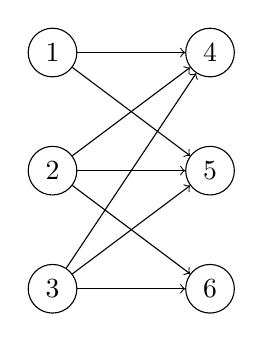
\begin{tikzpicture}              
            \node [circle, draw=black] (1) at (0, 3) {$1$};  
            \node [circle, draw=black] (2) at (0, 1.5) {$2$}; 
            \node [circle, draw=black] (3) at (0, 0) {$3$}; 
            \node [circle, draw=black] (4) at (2, 3) {$4$}; 
            \node [circle, draw=black] (5) at (2, 1.5) {$5$}; 
            \node [circle, draw=black] (6) at (2, 0) {$6$};

            \draw [->] (1) -- (4); \draw [->] (1) -- (5); 
            \draw [->] (2) -- (4); \draw [->] (2) -- (5); \draw [->] (2) -- (6);
            \draw [->] (3) -- (4); \draw [->] (3) -- (5); \draw [->] (3) -- (6);        
        \end{tikzpicture} 
    \end{center}
    This is almost a complete bipartite graph; it is only missing the edge 
    from job $1$ to job $6$. An optimal schedule is given below with 
    $C_{\max} = 3$. 
    \begin{center} 
        \begin{tikzpicture}[/pgfgantt/y unit chart=0.7cm] 
            \begin{ganttchart}[
                title/.style={draw=none},
                canvas/.append style={draw=none}, 
                bar top shift=0.1, bar height=0.6,
                y unit title=0.7cm,
            ]{1}{3}
                \ganttbar{Machine 1}{1}{2} \ganttbar[inline]{2}{1}{1} \ganttbar[inline]{1}{2}{2} \ganttbar[inline]{4}{3}{3} \\ 
                \ganttbar{Machine 2}{1}{2} \ganttbar[inline]{3}{1}{1} \ganttbar[inline]{6}{2}{2} \ganttbar[inline]{5}{3}{3}
            \end{ganttchart}
        \end{tikzpicture}
    \end{center}
    \vspace{-0.4cm}
    On the other hand, the CP rule could arbitrarily pick job $1$ to 
    be processed at time $0$, which would prevent job $6$ from running 
    at time $1$ as its predecessors are jobs $2$ and $3$. One such schedule 
    obtained from the CP rule is as follows, and it has $C_{\max} = 4$, 
    which matches the worst case bound above. 
    \begin{center} 
        \begin{tikzpicture}[/pgfgantt/y unit chart=0.7cm] 
            \begin{ganttchart}[
                title/.style={draw=none},
                canvas/.append style={draw=none}, 
                bar top shift=0.1, bar height=0.6,
                y unit title=0.7cm,
            ]{1}{3}
                \ganttbar{Machine 1}{1}{1} \ganttbar[inline]{1}{1}{1} \ganttbar[inline]{3}{2}{2} \ganttbar[inline]{4}{3}{3} \ganttbar[inline]{6}{4}{4} \\ 
                \ganttbar{Machine 2}{1}{1} \ganttbar[inline]{2}{1}{1} \ganttbar[inline]{5}{3}{3} 
            \end{ganttchart}
        \end{tikzpicture}
    \end{center}
\end{exmp}

Next, we give an example where LNS does not yield an optimal schedule for 
arbitrary precedence constraints. 

\begin{exmp}{exmp:6.12}
    Consider the instance of $(P_2~|~p_j=1, \text{prec}~|~C_{\max})$ 
    with precedence constraints given by the following directed acyclic 
    graph. 
    \begin{center}
        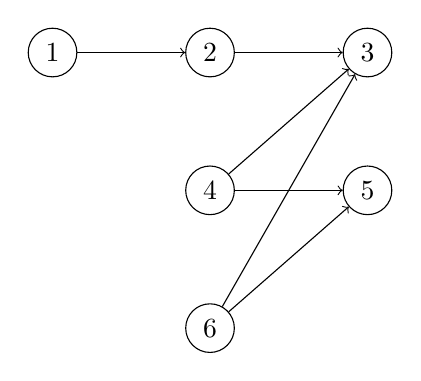
\begin{tikzpicture}              
            \node [circle, draw=black] (1) at (0, 3.5) {$1$};  
            \node [circle, draw=black] (2) at (2, 3.5) {$2$}; 
            \node [circle, draw=black] (3) at (4, 3.5) {$3$}; 
            \node [circle, draw=black] (4) at (2, 1.75) {$4$}; 
            \node [circle, draw=black] (5) at (4, 1.75) {$5$}; 
            \node [circle, draw=black] (6) at (2, 0) {$6$};

            \draw [->] (1) -- (2); \draw [->] (2) -- (3); 
            \draw [->] (4) -- (3); \draw [->] (4) -- (5);
            \draw [->] (6) -- (3); \draw [->] (6) -- (5);     
        \end{tikzpicture} 
    \end{center}
    \newpage
    An optimal schedule is given below with $C_{\max} = 3$. 
    \begin{center} 
        \begin{tikzpicture}[/pgfgantt/y unit chart=0.7cm] 
            \begin{ganttchart}[
                title/.style={draw=none},
                canvas/.append style={draw=none}, 
                bar top shift=0.1, bar height=0.6,
                y unit title=0.7cm,
            ]{1}{3}
                \ganttbar{Machine 1}{1}{2} \ganttbar[inline]{1}{1}{1} \ganttbar[inline]{2}{2}{2} \ganttbar[inline]{3}{3}{3} \\ 
                \ganttbar{Machine 2}{1}{2} \ganttbar[inline]{4}{1}{1} \ganttbar[inline]{6}{2}{2} \ganttbar[inline]{5}{3}{3}
            \end{ganttchart}
        \end{tikzpicture}
    \end{center}
    \vspace{-0.4cm}
    The LNS rule would pick jobs $4$ and $6$ first as they each have two 
    successors. This causes job $2$ to finish at time $3$ at the earliest, 
    preventing job $3$ from being run afterwards. So the LNS rule 
    yields a schedule with $C_{\max} = 4$. 
    \begin{center} 
        \begin{tikzpicture}[/pgfgantt/y unit chart=0.7cm] 
            \begin{ganttchart}[
                title/.style={draw=none},
                canvas/.append style={draw=none}, 
                bar top shift=0.1, bar height=0.6,
                y unit title=0.7cm,
            ]{1}{3}
                \ganttbar{Machine 1}{1}{2} \ganttbar[inline]{4}{1}{1} \ganttbar[inline]{1}{2}{2} \ganttbar[inline]{2}{3}{3} \ganttbar[inline]{3}{4}{4} \\ 
                \ganttbar{Machine 2}{1}{2} \ganttbar[inline]{6}{1}{1} \ganttbar[inline]{5}{2}{2} 
            \end{ganttchart}
        \end{tikzpicture}
    \end{center}
    \vspace{-0.4cm}
\end{exmp}

Both the CP rule and the LNS rule have more generalized versions that
can be applied to problems with arbitrary job processing times. Instead of
counting the number of jobs (as in the case with unit processing times), these
more generalized versions prioritize based on the total amount of processing
remaining to be done on the jobs in question. The CP rule then gives the
highest priority to the job that is heading the string of jobs with the largest
total amount of processing (with the processing time of the job itself also being
included in this total). The generalization of the LNS rule gives the highest
priority to that job that precedes the largest total amount of processing; again
the processing time of the job itself is also included in the total. The LNS name
is clearly not appropriate for this generalization with arbitrary processing times,
as it refers to a number of jobs rather than to a total amount of processing.

\subsection{Makespan with Machine Dependent Constraints} \label{subsec:6.3}
We consider another generalization of the $(P_m~||~C_{\max})$ problem 
where each job $j$ is only allowed to be run on a subset $M_j$ of the $m$ 
parallel machines. We will again consider the case with unit processing times, 
denoted by $(P_m~|~p_j=1, M_j~|~C_{\max})$. 

We note that this problem can be represented using a bipartite graph with $n$ 
edges $1, \dots, n$ corresponding to the jobs and $m$ edges $\text{mc}_1, 
\dots, \text{mc}_m$ corresponding to the machines. We place an edge 
$(j, \text{mc}_i)$ in the graph if and only if $i \in M_j$. 

We say that the sets $M_j$ are {\bf nested} if exactly one of the 
following conditions hold for any two jobs $j$ and $k$: 
\begin{enumerate}[(i)]
    \item $M_j = M_k$; 
    \item $M_j \subsetneq M_k$;
    \item $M_k \subsetneq M_j$; or 
    \item $M_j \cap M_k = \varnothing$.
\end{enumerate} 
When the sets $M_j$ are nested, the {\bf Least Flexible Job (LFJ)} rule 
plays an important role. 

\begin{algo}[Least Flexible Job (LFJ)]{algo:6.13}
    Every time a machine is freed, select among the available jobs the job 
    that can be processed on the \emph{smallest} number of machines. Ties 
    can be broken arbitrarily. 
\end{algo}

This rule is rather crude as it does not specify, for example, which
machine should be considered first when several machines become available at
the same time. It can be shown that the LFJ rule is optimal for 
$(P_m~|~p_j=1, M_j~|~C_{\max})$ when the sets $M_j$ are nested by using 
a standard interchange argument. In particular, when there are two 
machines, the sets $M_j$ are always nested, so the LFJ rule is optimal 
for $(P_2~|~p_j=1, M_j~|~C_{\max})$. However, in the case that $m \geq 3$ 
and the sets $M_j$ are arbitrary, the LFJ rule will not always yield an 
optimal schedule. We give an example of this below. 

\begin{exmp}{exmp:6.14}
    Consider the following instance of $(P_4~|~p_j=1, M_j~|~C_{\max})$ 
    with $n = 8$ jobs. 
    \begin{align*}
        \begin{array}{c|cccccccc}
            j & 1 & 2 & 3 & 4 & 5 & 6 & 7 & 8 \\ \hline 
            M_j & \{1,2\} & \{1,3,4\} & \{1,3,4\} & \{2\} & \{3,4\} 
            & \{3,4\} & \{3,4\} & \{3,4\}
        \end{array}
    \end{align*}
    It is clear that the sets $M_j$ are not nested by considering $M_1$ 
    and $M_2$. We now run the LFJ rule. Consider machine $1$ first. 
    The least flexible job that can be processed on machine $1$ is job $1$ 
    since it can be processed on only two machines, while jobs $2$ and $3$ 
    can be processed on three machines. The least flexible job to be processed 
    on machine $2$ is clearly job $4$. At time $0$, the least flexible jobs 
    to be processed on machines $3$ and $4$ could be jobs $5$ and $6$. 
    At time $1$, after jobs $1$, $4$, $5$, and $6$ have completed their processing 
    on the four machines, the least flexible job to be processed on machine 
    $1$ is job $2$. But none of the remaining jobs can be processed on 
    machine $2$, so it is forced to idle. The least flexible jobs to 
    go on machines $3$ and $4$ are jobs $7$ and $8$. Finally, job $3$ 
    can be run on machine $1$ at time $3$, so $C_{\max} = 3$. This schedule 
    is illustrated below. 
    \begin{center} 
        \begin{tikzpicture}[/pgfgantt/y unit chart=0.7cm] 
            \begin{ganttchart}[
                title/.style={draw=none},
                canvas/.append style={draw=none}, 
                bar top shift=0.1, bar height=0.6,
                y unit title=0.7cm,
            ]{1}{3}
                \ganttbar{Machine 1}{1}{1} \ganttbar[inline]{1}{1}{1} \ganttbar[inline]{2}{2}{2} \ganttbar[inline]{3}{3}{3} \\
                \ganttbar{Machine 2}{1}{1} \ganttbar[inline]{4}{1}{1} \\
                \ganttbar{Machine 3}{1}{1} \ganttbar[inline]{5}{1}{1} \ganttbar[inline]{7}{2}{2} \\ 
                \ganttbar{Machine 4}{1}{1} \ganttbar[inline]{6}{1}{1} \ganttbar[inline]{8}{2}{2}
            \end{ganttchart}
        \end{tikzpicture}
    \end{center}
    \vspace{-0.4cm}
    An optimal schedule with $C_{\max} = 2$ is given below, so LFJ was not optimal. 
    \begin{center} 
        \begin{tikzpicture}[/pgfgantt/y unit chart=0.7cm] 
            \begin{ganttchart}[
                title/.style={draw=none},
                canvas/.append style={draw=none}, 
                bar top shift=0.1, bar height=0.6,
                y unit title=0.7cm,
            ]{1}{3}
                \ganttbar{Machine 1}{1}{1} \ganttbar[inline]{2}{1}{1} \ganttbar[inline]{3}{2}{2} \\
                \ganttbar{Machine 2}{1}{1} \ganttbar[inline]{1}{1}{1} \ganttbar[inline]{4}{2}{2} \\
                \ganttbar{Machine 3}{1}{1} \ganttbar[inline]{5}{1}{1} \ganttbar[inline]{6}{2}{2} \\ 
                \ganttbar{Machine 4}{1}{1} \ganttbar[inline]{7}{1}{1} \ganttbar[inline]{8}{2}{2}
            \end{ganttchart}
        \end{tikzpicture}
    \end{center}
\end{exmp}

From Example~\ref{exmp:6.14}, one may expect that if a number of machines are 
free at the same point in time, it is advantageous to consider first the least 
flexible machine. The flexibility of a machine could be defined as the number 
of remaining jobs that can be processed (or the total amount of processing that 
can be done) on that machine. However, assigning any job to the {\bf Least 
Flexible Machine (LFM)} at each point in time does not guarantee an optimal
schedule in the case of Example~\ref{exmp:6.14}.

Heuristics can be designed that combine the LFJ rule with the LFM rule,
giving priority to the least flexible jobs on the least flexible machines. That is,
consider at each point in time first the Least Flexible Machine (LFM) (that is,
the machine that can process the smallest number of jobs) and assign to this
machine the least flexible job that can be processed on it. Any ties may be
broken arbitrarily. This heuristic may be referred to as the LFM-LFJ heuristic.
However, we find again that the LFM-LFJ does not yield an optimal schedule for 
Example~\ref{exmp:6.14}.

\subsection{Makespan with Preemptions} \label{subsec:6.4}
We now consider the same problem with preemptions allowed, namely the 
$(P_m~|~\text{prmp}~|~C_{\max})$ problem. Usually, but not always, allowing 
preemptions simplifies the analysis of a problem. This is indeed the case for 
this problem, where it actually turns out that many schedules are optimal. 
First, consider the following linear programming formulation of the problem, 
where $x_{ij}$ is the total time spent by machine $i$ on job $j$. 
\begin{align*}
    \min\quad & C_{\max} \\ 
    \text{s.t.}\quad & \sum_{i=1}^m x_{ij} = p_j, && j \in [n] \\ 
    & \sum_{i=1}^m x_{ij} \leq C_{\max}, && j \in [n] \\
    & \sum_{j=1}^n x_{ij} \leq C_{\max}, && i \in [m] \\
    & x_{ij} \geq 0, && i \in [m],\,j \in [n]. 
\end{align*}
The first set of constraints ensures that each job receives the required 
amount of processing. The second set of constraints ensures that the total 
amount of processing of each job is less than the makespan. The third 
set of constraints ensures that the total amount of processing on each 
machine is less than the makespan. Finally, the last constraint ensures that 
the execution fragments are non-negative. 

Since $C_{\max}$ is basically a decision variable and not an element of 
the resource vector of the linear program, we can rewrite the second and third 
set of constraints as 
\begin{align*}
    C_{\max} - \sum_{i=1}^m x_{ij} &\geq 0, && j \in [n] \\ 
    C_{\max} - \sum_{j=1}^n x_{ij} &\geq 0, && i \in [m]. 
\end{align*}
This LP can be solved in polynomial time, but the solution of the LP does
not prescribe an actual schedule; it merely specifies the amount of time job
$j$ should spend on machine $i$. However, with this information, a schedule can
easily be constructed.

We consider another algorithm for $(P_m~|~\text{prmp}~|~C_{\max})$. This 
algorithm is based on the fact that it is easy to obtain an expression for the
makespan under the optimal schedule. In the next lemma, we establish a lower 
bound. We leave its proof as an exercise. 

\begin{lemma}{lemma:6.15}
    Under the optimal schedule for $(P_m~|~\text{prmp}~|~C_{\max})$, we have 
    \[ C_{\max} \geq \max\left( p_1, \frac1m \sum_{j=1}^n p_j \right) 
    =: C^*_{\max}. \] 
\end{lemma}

Having a lower bound allows for the construction of a very simple algorithm
that minimizes the makespan. The fact that this algorithm actually produces
a schedule with a makespan that is equal to the lower bound shows that the
algorithm yields an optimal schedule.

\begin{algo}[Minimizing Makespan with Preemptions]{algo:6.16}
    \begin{enumerate}
        \item Take the $n$ jobs and process them one after another on a single 
        machine in any sequence (that is, without preemption). The makespan is 
        then equal to the sum of the $n$ processing times and is at most 
        $m \cdot C^*_{\max}$.
        
        \item Take this single machine schedule and divide it into $m$ equal parts.
        
        \item Execute each of the $m$ parts in Step 2 on a separate machine. 
    \end{enumerate}
\end{algo}

It is clear that the resulting schedule is feasible. Part of a job may appear
at the end of the schedule for machine $i$ while the remaining part may appear
at the beginning of the schedule for machine $i + 1$. As preemptions are allowed
and the processing time of each job is less than $C^*_{\max}$, such a schedule 
is feasible. Moreover, this schedule as $C_{\max} = C^*_{\max}$, so it is 
also optimal. 